\documentclass{article}
\usepackage{../fasy-hw}

%% UPDATE these variables:
\renewcommand{\hwnum}{7}
\title{Advanced Algorithms, Homework \hwnum}
\author{Ben Miller}
\collab{\todo{list your collaborators here}}
\date{due: Monday, 8 December 2021}

\begin{document}

\maketitle

This homework assignment should be
submitted as a single PDF file both to D2L and to Gradescope.

General homework expectations:
\begin{itemize}
    \item Homework should be typeset using LaTex.
    \item Answers should be in complete sentences and proofread.
    \item You will not plagiarize, nor will you share your written solutions
        with classmates.
    \item List collaborators at the start of each question using the
        \texttt{collab} command.
    \item Put your answers where the \texttt{todo} command currently is (and
        remove the \texttt{todo}, but not the word \texttt{Answer}).
    \item If you are asked to come up with an algorithm, you are
        expected to give an algorithm that beats the brute force (and, if possible, of
        optimal time complexity). With your algorithm, please provide the following:
        \begin{itemize}
            \item \emph{What}: A prose explanation of the problem and the algorithm,
                including a description of the input/output.
            \item \emph{How}: Describe how the algorithm works, including giving
                psuedocode for it.  Be sure to reference the pseudocode
                from within the prose explanation.
            \item \emph{How Fast}: Runtime, along with justification.  (Or, in the
                extreme, a proof of termination).
            \item \emph{Why}: Statement of the loop invariant for each loop, or
                recursion invariant for each recursive function.
        \end{itemize}
\end{itemize}


\collab{}
\nextprob{}

The \texttt{rand()} function in the standard C library returns a
uniformly random number in \texttt{[0,RANDMAX-1]}. Does \texttt{rand}()$\mod n$
generate a number uniformly distributed in $[0,n-1]$? (Prove or disprove).

% Note I: This is the second variant in EPI 5.12.

\paragraph{Answer}
No, \texttt{rand}()$\mod n$ will not generate a number uniformly distributed in
$[0,n-1]$. This would only work in the case where RANDMAX was a multiple of n.

Let us consider the case where RANDMAX = 5 and n = 3. Let A = a set of numbers from
0 to 4. By appliying $\mod n$ to each number in A, we get [0, 1, 2, 0, 1], which
gives us the frequencies [2,2,1]. Because the rand function is uniformly destributed,
this transform will not be uniformly distributed.

If we apply the same process with RANDMAX = 6 and n = 3, we get a frequency list of
[2,2,2]. In the general case where RANDMAX is a multiple of n, the distribution of
\texttt{rand}()$\mod n$ will be uniform.

Therefore, \texttt{rand}()$\mod n$ will not always be uniformly distributed.



\collab{}
\nextprob{}

Algorithms where we use randomization to find a deterministic answer are known
as Las Vegas algorithms.  Monte Carlo algorithms also use randomization, but
might not always give the right answer; however, they either have a high
probability of being correct or close to correct.

\begin{enumerate}[(a)]
    \item Give a Monte Carlo algorithm to estimate~$\pi$.
    \item Let $n$ be the number of random numbers used by your algorithm.
        Explain why as $n \to \infty$, the expectation of the output for your
        algorithm is~$\pi$.
    \item Implement this algorithm and plot a line graph of
        the values returned for at least $10$ values of~$n$.
\end{enumerate}

Note: Assume that there is a function \texttt{randReal}$[a,b]$ that returns a random
real number between $a$ and $b$, iid from the uniform distribution over the
interval $[a,b]$.

\paragraph{Answer}
We create a one by one square and inscribe a circle. From all the random points
given, we map them to coordinates in the square. The ratio of points in the circle
to all points will approximate a proportion of pi.

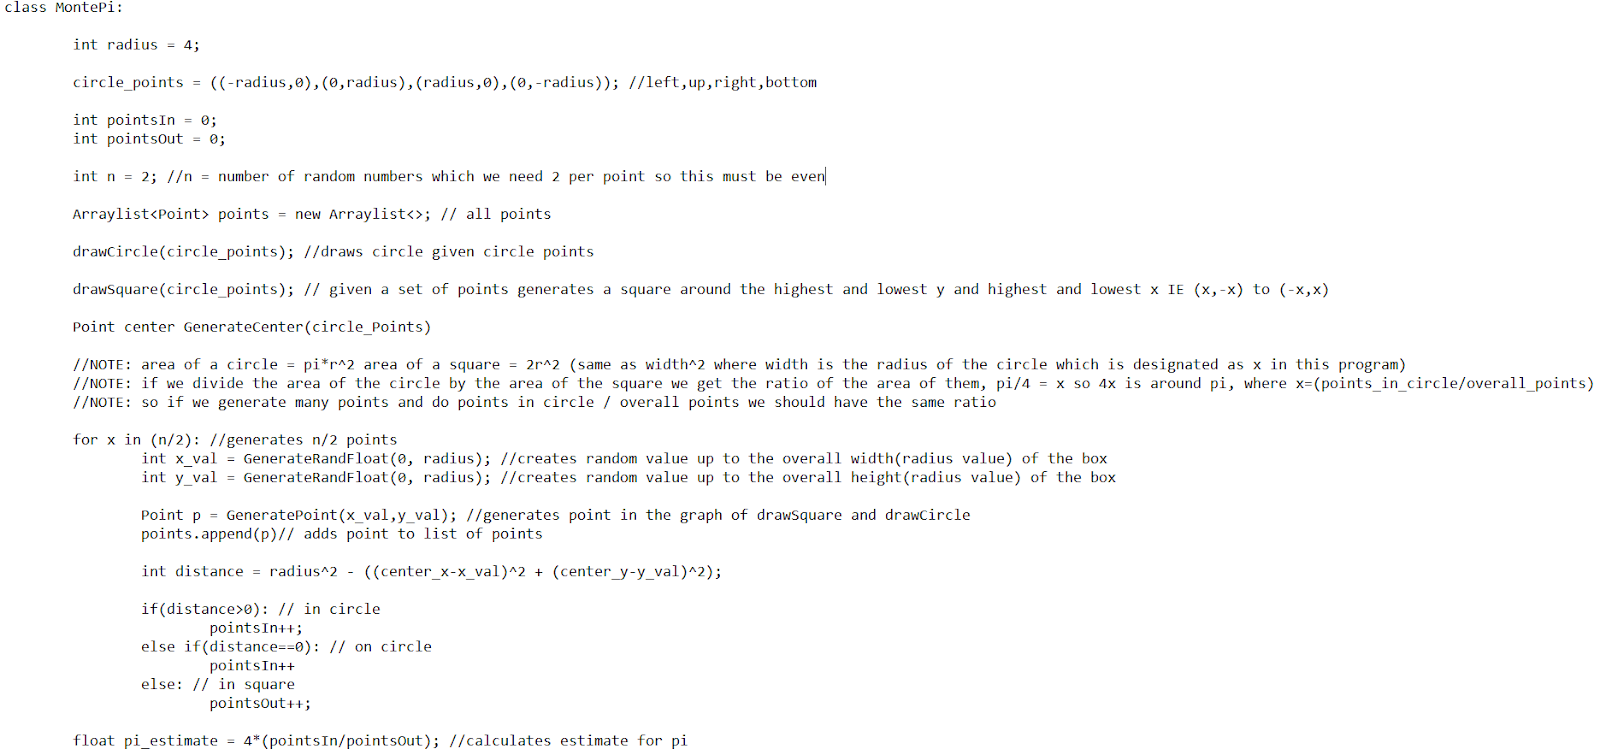
\includegraphics[width=500,height=500,keepaspectratio]{q2Code.png}

Part b:
The reason that as n moves towards infinity we get better approximations of pi is that since we will have increasingly many points the approximation made will be better since in the bottom you can see we estimate pi based on 4*(pointsIn/pointsOut) with the reasoning listed in the notes above in the program. And it will follow the ratio of circle in the square.

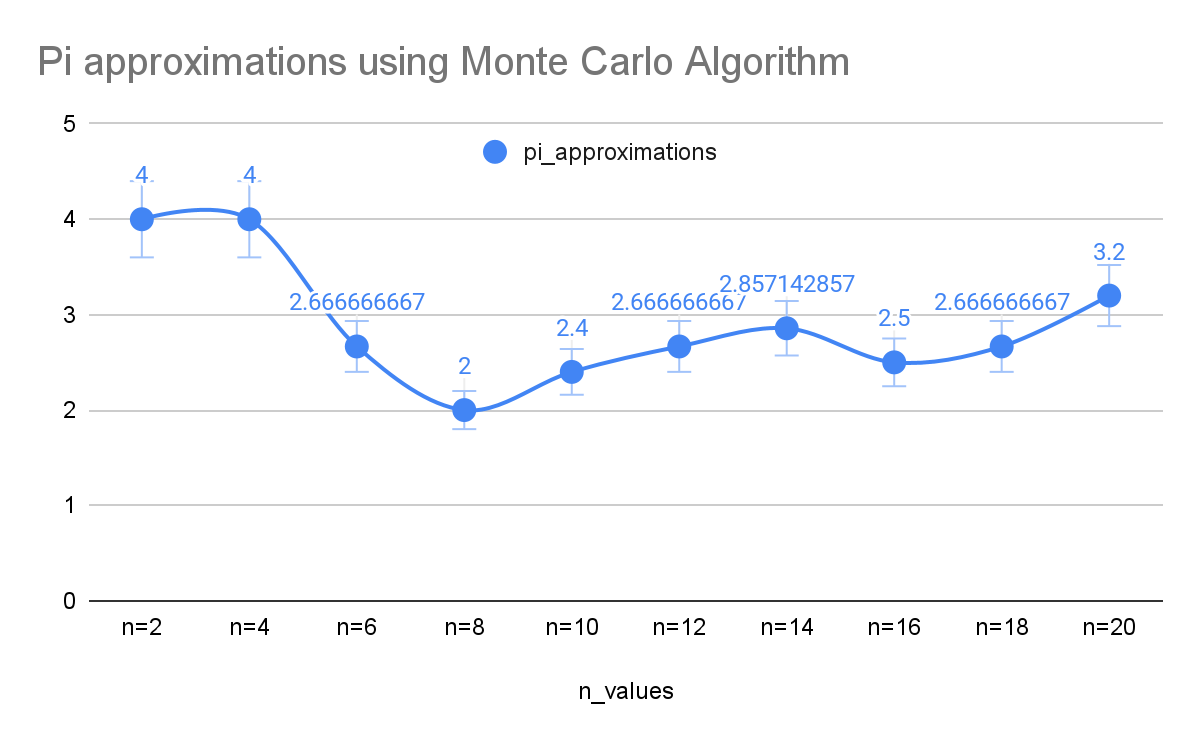
\includegraphics[width=500,height=500,keepaspectratio]{piCalcGraph.png}

\collab{}
\nextprob{}

Choose an algorithm that you analyzed on a homework in this class (can be this
HW or a previous one).  Suppose you are a journalist writing about this
break-through algorithm and write a one-page summary of the algorithm for a
general audience.  Describing the problem that this algorithm solves and the
applications of the problem should be highlighted (feel free to do some
research).  Detail of the algorithm and proofs of correctness or runtime should
be only given at a very high level.

\paragraph{Answer}

Kruskal's algorithm is no Krusty Krab!\\
Discovered in 1956 \footnote{Used information from the textbook}

Think about how many networks there are in the world. From roads to irrigation, telephone wires to sewage pipes, railroads to newspapers, networks are a huge part of the world's infrastructure. The world is vast and infrastructure is expensive. Joseph Kruskal has just published a new "Minimum Spanning Tree" algorithm that will drastically reduce spending everywhere.

Any network can be broken down into vertices and edges. For this example, lets work with telephone cables within a state. A city or town is a vertex, and a path connecting them is an edge. We are not immediately concerned with capacities here, yet, so it would theoretically be fine if all traffic were to go through one edge. There is no point in connecting a city to another city through two paths, which makes this network a “tree.”

Installing all of those cables requires a lot of money for materials and equipment and a lot of training and hours to build. Not to mention maintenance! The problem here is to minimize the amount of cable laid to maximize profits and minimize downtime in the case of an outage. We need to install those cables and span all the cities with minimal material. Thus, we get a minimum spanning tree.

The core idea behind this algorithm is really quite simple, but the hard part is the proof. Kruskal’s algorithm can be boiled down to one simple statement. “Scan all edges by increasing weight; if an edge is safe, add it to the tree.” A safe edge is just an edge that won’t make a loop in the network, which would make it not a tree anymore.

The algorithm is quite fast for most applications. If we were running this algorithm on a massive network with millions of edges, say a complex, statewide sewer system, it could take a while to run! The overall running time of Kruskal’s algorithm is O(E log V), with the longest part of the algorithm being the initial sorting of the edges. This running time is really good, and it certainly shouldn’t slow down any development plans.

Real world scenarios sometimes require there to be loops in networks, capacities can become a problem, or managing a large channel can become expensive. A tree is just not fit for all applications. A minimum spanning tree can still be a great place to start. New edges can be added in after an initial base is completed, or some edges in the current minimum spanning tree can be removed and a second tree can be calculated and combined with the first. Although not directly applicable to tons of areas, a minimum spanning tree can serve as an algorithmically optimal base from which to plan the final network.

Feedback from friend:

"I don't know what you are talking about really, but I love the enthusiasm! Descriptive language is nice!" I tried to write the page to be impactful rather than straight forward, which does make it harder to see what I'm actually talking about.

\collab{\todo{}}
\nextprob{Removing an Edge}

Chapter 8, Question 4, Part(a)

For any edge e in any graph G, let G minus e denote the graph obtained by
deleting e from G. Suppose we are given a graph G and two vertices s
and t. The replacement paths problem asks us to compute the shortest-path
distance from s to t in G minus e, for every edge e of G. The output is an array
of E distances, one for each edge of G.

(a) Suppose G is a directed graph, and the shortest path from vertex s to
vertex t passes through every vertex of G. Describe an algorithm to solve
this special case of the replacement paths problem in O(E log V ) time.

\paragraph{Answer}
Because the shortest path from vertex s to vertex t passes through every vertex
of G, we know that the shortest path minus e lies on some path that goes through
a subset of the vertices up to e and a subset of the vertices after e. So, if
an edge is taken out of the shortest path, we will walk back from the edge that was
taken out and we will try every edge that connects to the path after the missing
edge to see if it is shorter.

\begin{algorithm} \caption{\textsc{RemoveEdges} (G)}\label{alg:seb}
    {\bf Input:} directed graph\\
    {\bf Output:} array of E distances
    \begin{algorithmic}[1]
        \State$Path \gets Djikstra\ shortest\ path$
        \State$EArray \gets array\ with\ length\ |E|$
        \State$NotInPathSet \gets new\ set$
        \For{$edge\ e \in E$}
            \If{$e \notin Path$}
                \State$EArray[e] \gets len(Path)$
            \Else{}
                \State$NotInPathSet\ add\ e$
            \EndIf{}
        \EndFor{}
        \For{$e \in NotInPathSet$}
            % \State$tempNotInPathSet \gets new\ set$
            \State$shortestPath \gets \infty$
            \State$curVertex \gets vertex\ before\ e$
            \For{$f \in edges\ from\ curVertex\ to\ vertex\ after\ e$}
            \State$newLen \gets len(Path\ to\ curVertex) + f + len(Path\ from\ f\ to\ t) $
                \If{$newLen < shortestPath$}
                \State$ShortestPath \gets newLen$
                \EndIf{}
                \State$EArray[e] \gets newLen$
            \EndFor{}
        \EndFor{}
        \State$return\ EArray$
    \end{algorithmic}
\end{algorithm}

With our nifty knowledge that the shortest path passes through every vertex, we
are able to calculate the shortest path for each edge removed in $O(E log V)$ time.

We can put each edge that is in the shortest path found by an initial djikstra run into a set. Then, we can check whether each edge is in that set in constant time. If the edge is not in that set, updating EArray for removing that edge takes constant time. If the edge is in that set, it takes $O(E log V)$ time. There are E edges that we need to check, so the overall running time is $O(E (E log V))$.

\collab{\todo{}}
\nextprob{}

Chapter 10, Question 4, (Opposing Edges)
Let G be a flow network that contains an opposing pair of edges u  v and
v  u, both with positive capacity. Let G 0 be the flow network obtained from G
by decreasing the capacities of both of these edges by min{c(u  v), c(v  u)}.
In other words:

• If c(u  v) > c(v  u), change the capacity of u  v to c(u  v) − c(v  u)
and delete v  u.
344Exercises

• If c(u  v) < c(v  u), change the capacity of v  u to c(v  u) − c(u  v)
and delete u  v.

• Finally, if c(u  v) = c(v  u), delete both u  v and v  u.

(a) Prove that every maximum (s, t)-flow in G 0 is also a maximum (s, t)-flow
in G. (Thus, by simplifying every opposing pair of edges in G, we obtain
a new reduced flow network with the same maximum flow value as G.)

(b) Prove that every minimum (s, t)-cut in G is also a minimum (s, t)-cut
in G 0 and vice versa.

(c) Prove that there is at least one maximum (s, t)-flow in G that is not a
maximum (s, t)-flow in G 0

\paragraph{Answer}

Choose the maximum edge and reduce it by the minimum edge. Remove the minimum edge

\todo{answer here}

\collab{}
\nextprob{}

Chapter 11, Question 6, (Mini-Golf)

The SPU Commuter Silence Department is installing a mini-golf course in
the basement of the See-Bull Center! The playing field is a closed polygon
bounded by m horizontal and vertical line segments, meeting at right angles.
The course has n starting points and n holes, in one-to-one correspondence.
It is always possible hit the ball along a straight line directly from each
starting point to the corresponding hole, without touching the boundary
of the playing field. (Players are not allowed to bounce golf balls off the
walls; too much glass.) The n starting points and n holes are all at distinct
locations.

Sadly, the architect’s computer crashed just as construction was about to
begin. Thanks to the herculean efforts of their sysadmins, they were able to
recover the locations of the starting points and the holes, but all information
about which starting points correspond to which holes was lost!
Describe and analyze an algorithm to compute a one-to-one correspon-
dence between the starting points and the holes that meets the straight-line
requirement, or to report that no such correspondence exists. The input
consists of the x- and y-coordinates of the m corners of the playing field, the
n starting points, and the n holes. Assume you can determine in constant
time whether two line segments intersect, given the x- and y-coordinates
of their endpoints.

\paragraph{Answer}

A backtracking algorithm truly makes the most sense to me even though I know this
is an application of flows and cuts

I am taking inspiration from the algorithm given in Algorithms (Jeff Erickson) 11.4 for this problem.

To solve this problem with maximum flows, we will first hook up all holes to all starts
with a capacity of one where each edge is a possible connection (no connections go through walls). Then, we connect a vertex s to each start and a vertex t to each hole. Finally, to ensure that each vertex has a capacity of one, we convert each vertex in holes and starts to two vertices. The incoming edges are directed to one vertex, an edge with capacity of one connects to the other vertex, and all outgoing edges connect to that outgoing vertex. Then, we run a maximum flow between s and t. If the value of the maximum flow is less than the total number of starts or holes, then there is not a possible matching.

\begin{algorithm} \caption{\textsc{GolfPairing} (Corners, Starts, Holes)}\label{alg:seb}
    {\bf Input:} x,y coordinates of corners, starts, and holes\\
    {\bf Output:} one to one pairing between starts and holes
    \begin{algorithmic}[1]
        \State$Graph \gets\ Set\ up\ graph$
	\State$Flow \gets\ JohnHopcroftRichardKarpBipartiteMatching(Graph)$
	\If$|Flow| < size(starts)$
		\State$return\ no\ matching\ exists$
	\EndIf{}
	\State$return\ each\ disjoint\ path\ \in Flow - s\ and\ t$
    \end{algorithmic}
\end{algorithm}

To set up the graph, we have to calculate whether an edge is possible for each pair of start and hole vertices. We check that by seeing if the connecting line intersects with any of the lines from the course, which has M corners. This runs in $\Theta((N+M)^2)$ time. Performing the vertex transposition and hooking up s and t will run in $\Theta(N)$ time.

The book references a maximum bipartite matching that runs in $O( V^{½} E)$ time, so we could use that algorithm to achieve that runtime for the matching section. The $\Theta(N^2)$ step dominates the algorithm, so the overall running time runs in $\Theta((N+M)^2)$ time.

The algorithm for finding the matching itself revolves around finding alternating paths, then merging those paths with the symmetric difference with the flow.

\end{document}
